\documentclass[14pt]{beamer}

\usepackage[french]{babel}
\usepackage[T1]{fontenc}
\usepackage[utf8]{inputenc}

\newcommand\rae{$\rightarrow$ }
\newenvironment{framentitle}[1]
{
\begin{frame}
  \frametitle{#1}
}
{
\end{frame}
}


\usetheme{Singapore}
\setbeamertemplate{navigation symbols}{}
\setbeamertemplate{mini frames}{}

\title{UTC504 -- Systèmes d'Information et Bases de Données}
\subtitle{Introduction}
\author{Sébastien Fourestier}
\date{2022}


\begin{document}

\frame{\titlepage}

\begin{framentitle}{Bibliographie}
    \begin{itemize}
        \item Pascal \textsc{André}, Alain \textsc{Vally}: \emph{Conception des systèmes
            d'information}
        \item Jacqes \textsc{Printz}: \emph{Le genie logiciel}
        \item Florence \textsc{Petit}: \emph{Cycle de vie des
            systèmes informatiques}
        \item František Kardoš : Conception de systèmes d'information
        \item Pierre Gérard : UML, Diagrammes de classe
        \item \url{www.editions-eni.fr}: \emph{Cycle en spirale}
    \end{itemize}
\end{framentitle}

\begin{framentitle}{Correctifs}
    \begin{itemize}
        \item Ce cours est disponible sous licence libre sur ce dépôt github:\\
            \small{\url{https://github.com/sfourestier/enseignement}}
        \item[\ra] Voici pouvez :
            \begin{itemize}
                \item L'améliorer en proposant des \emph{Pull requests}
                \item Partager autour de points pouvant être améliorés en créant des
                    tickets (\emph{Issues})
            \end{itemize}
    \end{itemize}
\end{framentitle}

\begin{frame}
    \frametitle{Plan}
    \tableofcontents
\end{frame}

\section{Définitions}

\AtBeginSection[]
{
  \begin{frame}<beamer>
    \frametitle{Plan}
    \tableofcontents[currentsection]
%    \tableofcontents[currentsection,currentsubsection]
  \end{frame}
}

\begin{framentitle}{Introduction}
    \begin{itemize}
        \item Petits systèmes autonomes :
            \begin{itemize}
                \item Développement aisé et court
            \end{itemize}
        \item Accroissement des problèmes traités et diversité des domaines
            d'application de l'informatique
        \item[\ra] Systèmes complexes :
            \begin{itemize}
                \item Période de développement et durées de vie allongées
                \item Le développement est investissement durable
            \end{itemize}
        \item[\ra] Rentabiliser le développement et les efforts produits
    \end{itemize}
\end{framentitle}

\begin{framentitle}{Le génie logiciel (1)}
    Définition du génie logiciel au Journal officiel du 19 février 1984 :\\~
    \begin{quote}
        « l'ensemble des activités de conception et de mise en œuvre des
        produits et des procédures tendant à rationaliser la production du
        logiciel et son suivi »
    \end{quote}
\end{framentitle}

\begin{framentitle}{Le génie logiciel (2)}
    Définition adaptée de Jacques Printz :\\~
    \begin{quote}
        « l'ensemble des moyens techniques, industriels, industriels et humains
        qu'il faut réunir pour spécifier, construire, distribuer et maintenir
        des logiciels de qualité »
    \end{quote}
\end{framentitle}

\begin{framentitle}{Le génie logiciel (3)}
    Premiers critères de qualité :
    \begin{itemize}
        \item Sûrs :
            \begin{itemize}
                \item Réagissent de façon déterministe aux sollicitations
            \end{itemize}
        \item Conviviaux :
            \begin{itemize}
                \item Adaptés aux capacités des usagers
            \end{itemize}
        \item Évolutifs :
            \begin{itemize}
                \item S'adaptent aux nouveaux besoins
            \end{itemize}
        \item Économiques :
            \begin{itemize}
                \item Réalisent l'optimum entre le service rendu et les coûts de
                    développement/maintenance
            \end{itemize}
    \end{itemize}
\end{framentitle}

\begin{framentitle}{Système d'information (1)}
    Définition de Wikipédia :\\~
    \begin{quote}
        « Un système d'information (SI) est un ensemble organisé de ressources
        qui permet de collecter, stocker, traiter et distribuer de
        l'information. »
    \end{quote}
\end{framentitle}

\begin{framentitle}{Système d'information (2)}
    Définition adaptée de C. Rolland :
    \begin{itemize}
        \item Un Système d'information est un objet artificiel greffé sur un
            objet naturel (organisation, processus industriel, commande
            embarquée, etc.)
    \item Il est conçu pour mémoriser un ensemble d'images de l'objet réel à
        différents moments de sa vie
    \item Ces images doivent être accessibles par les partenaires de
        l'organisation pour décider des actions à entreprendre
    \end{itemize}
\end{framentitle}

\begin{framentitle}{Classification des SI}
    \begin{enumerate}
        \item SI de gestion :
            \begin{itemize}
                \item Beaucoup de données : consultation, mise à
                    jour
                \item Possibilité d'accès distant (réseau)
                \item Ex : gestion de clientèle, du stock, etc.
            \end{itemize}
        \item Le calcul scientifique :
            \begin{itemize}
                \item Beaucoup de calculs, peu de données
                \item Critère important : rapidité de traitement
                \item Ex : simulation, météo, imagerie
            \end{itemize}
        \item L'informatique temps réel :
            \begin{itemize}
                \item Critère important : réactivité du SI
                \item Informatique embarquée, contrôle de
                    processus (fabrication, surveillance), réseaux informatiques
                \item Ex : pilotage auto d'un avion, centrale nucléaire
            \end{itemize}
    \end{enumerate}
\end{framentitle}

\section{Modélisation}

\begin{framentitle}{Modélisation et développement}
    Pour développer des SI, on utilise des modèles :
    \begin{itemize}
        \item Modèle :
            \begin{itemize}
                \item Interprétation par son utilisateur de l'idée qu'il se
                    fait d'une situation
            \end{itemize}
        \item Développement :
            \begin{itemize}
                \item Le développement est une suite de modèles de plus en plus
                    précise (avec de moins en moins d'éléments laissés libres)
                \item[\ra] Lorsque tous les éléments ont été fixés, le SI est implémenté
            \end{itemize}
    \end{itemize}
\end{framentitle}

\begin{framentitle}{Méthodes de développement}
    Plusieurs types de processus de développement :
    \begin{itemize}
        \item Méthodes cartésiennes : « Diviser pour régner »
            \begin{itemize}
                \item On découpe en sous-éléments, on résout, on rassemble
                \item Ex : approche Objet
                \item Processus de développement :
                    \begin{itemize}
                        \item Basé sur les fonctionnalités
                    \end{itemize}
            \end{itemize}
        \item Méthodes systémiques : vision globale
            \begin{itemize}
                \item Compréhension des éléments et leurs relations
                \item Ex : Bases de données, Merise
                \item Processus de développement :
                    \begin{itemize}
                        \item Approche conceptuelle, par niveaux d'abstraction
                    \end{itemize}
            \end{itemize}
    \end{itemize}
\end{framentitle}

\begin{framentitle}{Exemple approche Objet}
    \begin{center}
    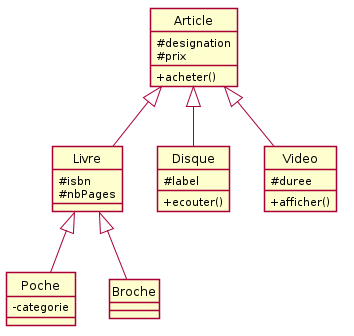
\includegraphics[width=.7\textwidth]{fig9.png}
    \end{center}
\end{framentitle}

\begin{framentitle}{Exemple approche Merise}
    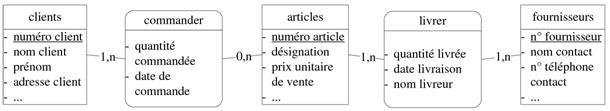
\includegraphics[width=\textwidth]{fig10.jpg}
\end{framentitle}

\begin{framentitle}{Trois axes de modélisation (1)}
    Un système d'information comprend 3 aspects :
    \begin{enumerate}
        \item Données :
            \begin{itemize}
                \item Ce que le système manipule
            \end{itemize}
        \item Comportement dynamique :
            \begin{itemize}
                \item Comment s'enchaînent les événements
            \end{itemize}
        \item Comportement fonctionnel :
            \begin{itemize}
                \item Quelles sont ses fonctionnalités
            \end{itemize}
    \end{enumerate}
\end{framentitle}

\begin{framentitle}{Trois axes de modélisation (2)}
    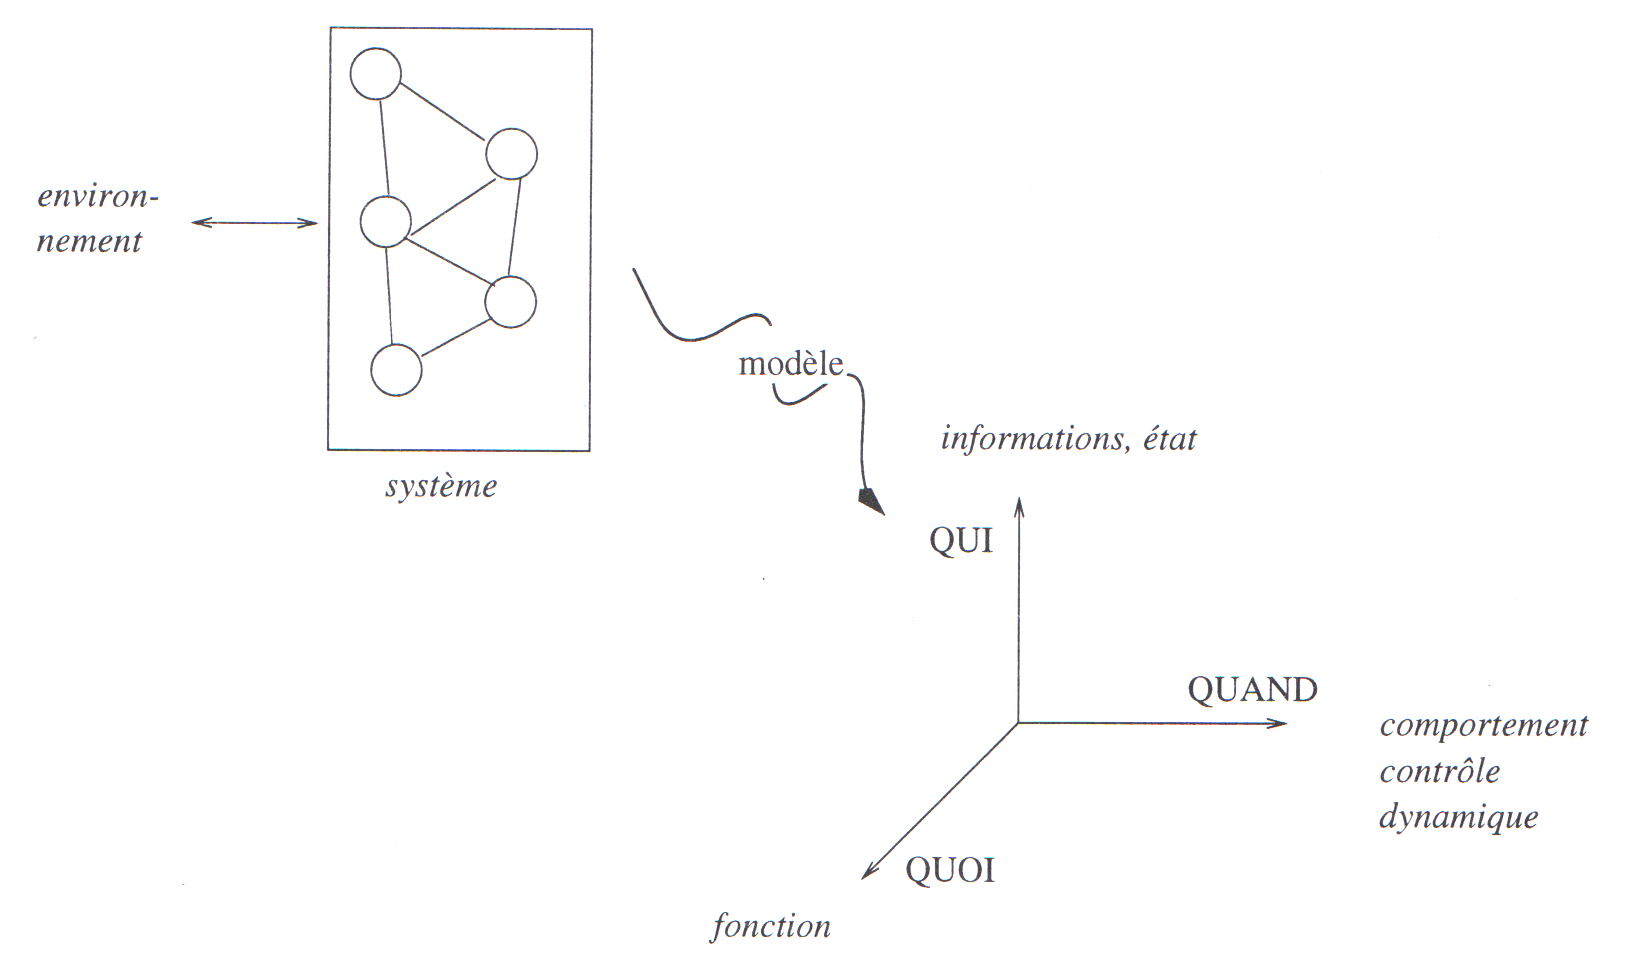
\includegraphics[width=\textwidth]{fig2.png}
    \rae Trois courants de méthodes d'analyse/conception
\end{framentitle}


\begin{framentitle}{Approche fonctionnelle}
    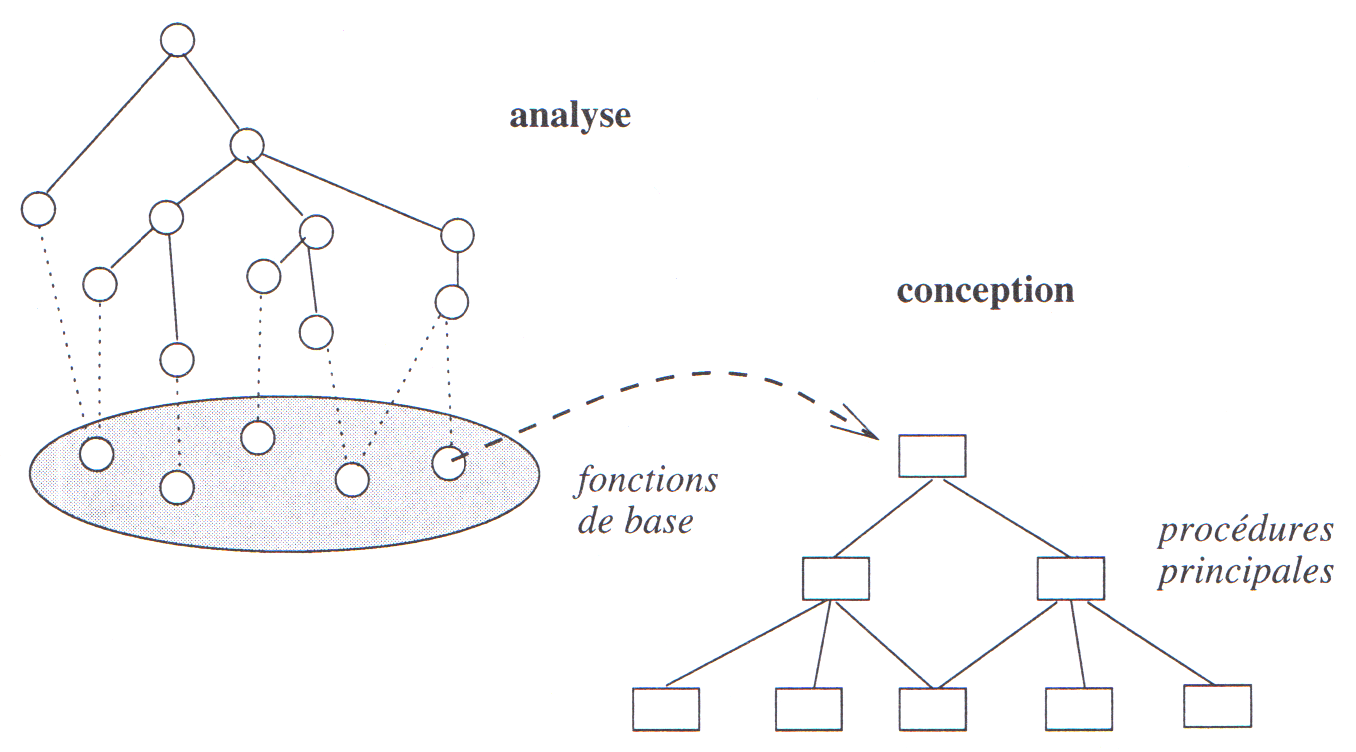
\includegraphics[width=\textwidth]{fig1b.png}
\end{framentitle}

\begin{framentitle}{Approche flots de données}
    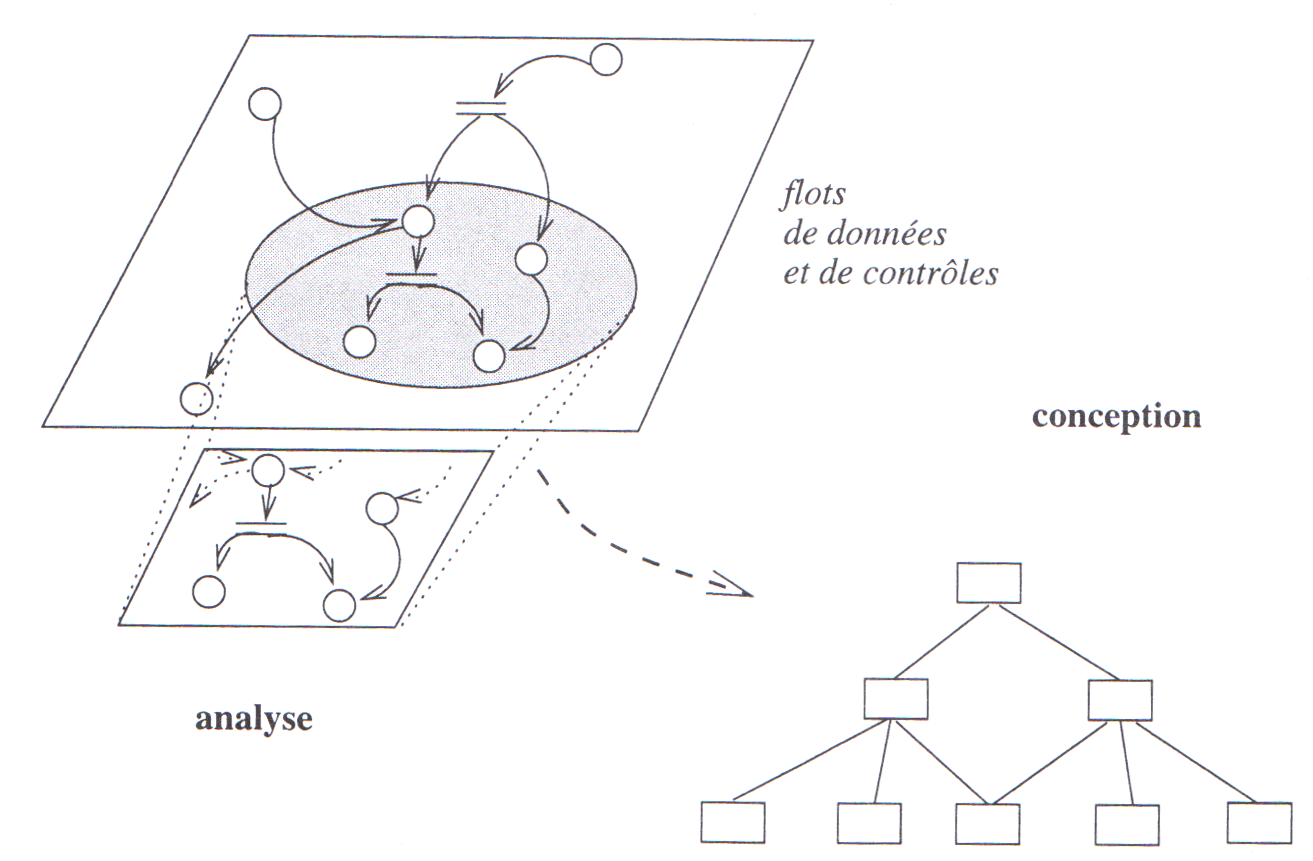
\includegraphics[width=\textwidth]{fig3a.png}
\end{framentitle}

\begin{framentitle}{Approche modèle de données}
    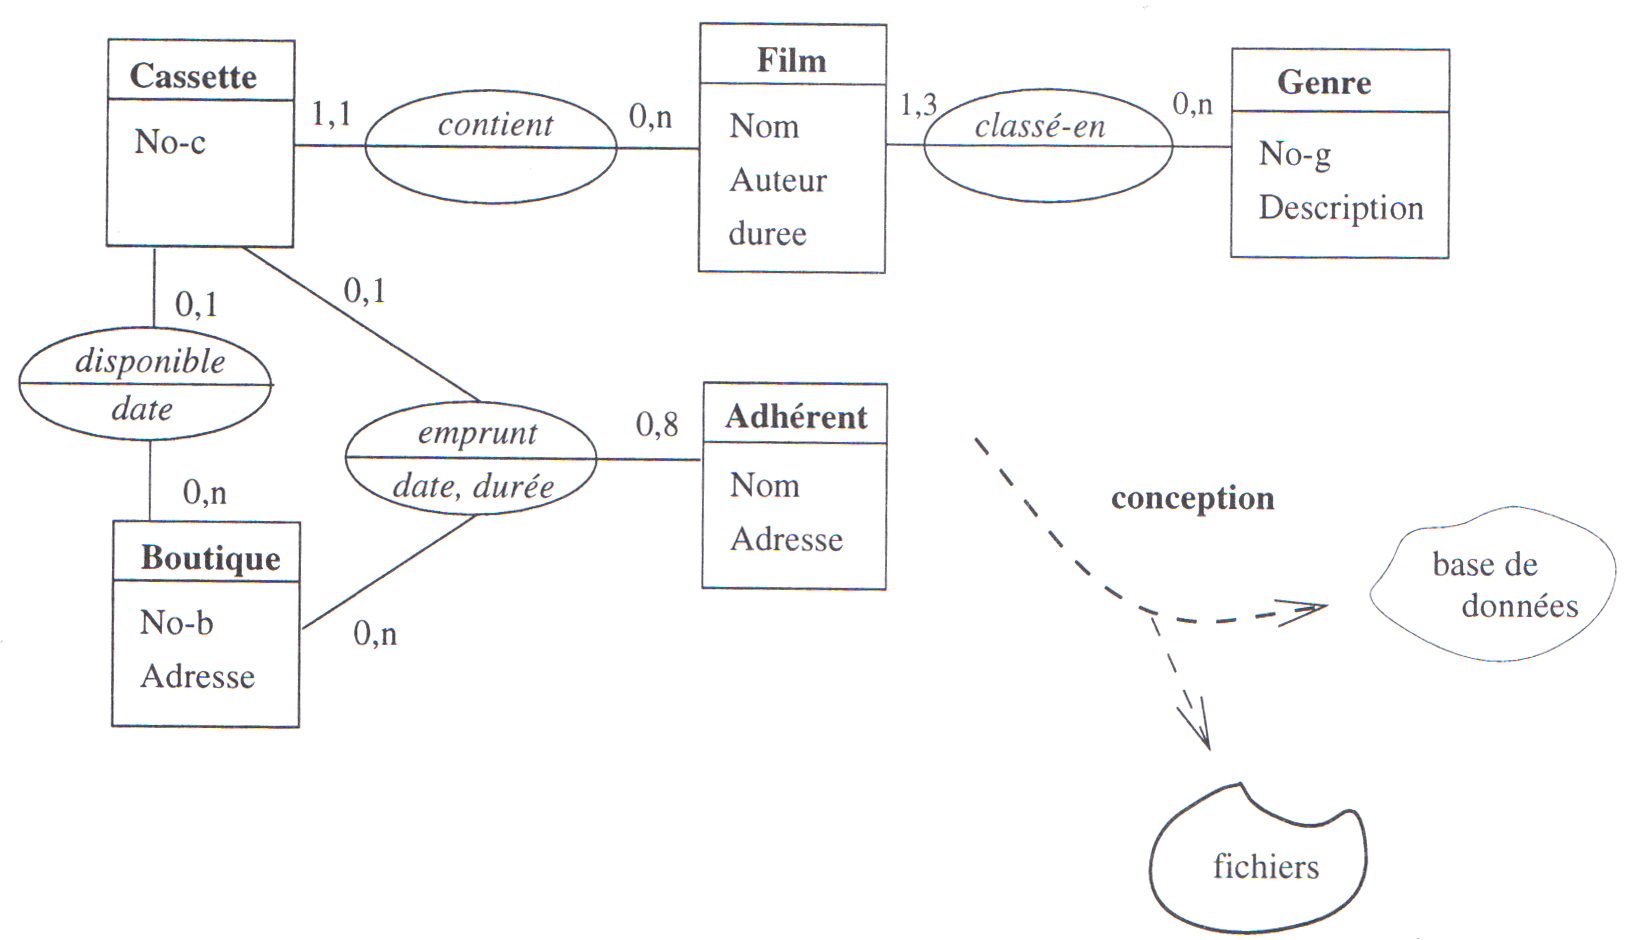
\includegraphics[width=\textwidth]{fig3b.png}
\end{framentitle}

\section{Étapes de développement}
\begin{frame}
    \frametitle{Étapes de développement des logiciels}
    \begin{enumerate}
        \item Analyse des besoins :
            \begin{itemize}
                \item Objectif du logiciel
            \end{itemize}
        \item Analyse :
            \begin{itemize}
                \item Expression des besoins
            \end{itemize}
        \item Conception :
            \begin{itemize}
                \item Proposition de solutions
            \end{itemize}
        \item Réalisation et Test :
            \begin{itemize}
                \item Production du programme
            \end{itemize}
        \item Installation :
            \begin{itemize}
                \item Mise en place dans l'organisation
            \end{itemize}
        \item Maintenance :
            \begin{itemize}
                \item Adaptation du logiciel et corrections
            \end{itemize}
    \end{enumerate}
\end{frame}

\begin{framentitle}{Étape 1/6 : Analyse des besoins}
    Objectif du logiciel:
    \begin{itemize}
        \item Phase initiale du développement
        \item Description et une évaluation globale des besoins
        \item Prend en compte :
            \begin{itemize}
                \item Les aspects économiques
                \item Les risques
                \item La compétitivité
                \item L'organisation globale du projet
            \end{itemize}
    \end{itemize}
\end{framentitle}

\begin{framentitle}{Étape 2/6 : Analyse}
    Expression des besoins:
    \begin{itemize}
        \item Écriture des fonctions que le logiciel doit effectuer et le
            contexte\\
            (conditions d'exploitation, qualité requise, etc.)
        \item Fait abstraction de la façon dont les fonctionnalités seront
            réalisée
    \end{itemize}
\end{framentitle}

\begin{framentitle}{Étape 3/6 : Conception}
    \begin{itemize}
        \item Définir de façon très précise :
            \begin{itemize}
                \item Les fonctionnalités
                \item L'architecture du logiciel
            \end{itemize}
        \item À partir :
            \begin{itemize}
                \item Des besoins exprimés
                \item Des contraintes générales définies dans les deux première
                    phases
            \end{itemize}
        \item La spécification peut être :
            \begin{itemize}
                \item Informelle, en langage naturel
                \item À l'aide de diagrammes
                \item Sur les 3 axes évoqués précédemment
            \end{itemize}
    \end{itemize}
\end{framentitle}

\begin{framentitle}{Étape 4/6 : Réalisation et Test}
    \begin{itemize}
        \item Phase de programmation
        \item Tests qui prouvent la logique du programme
            \begin{itemize}
                \item Tests unitaires :
                    \begin{itemize}
                        \item Validation des parties du logiciel (fonctions,
                            modules)
                    \end{itemize}
                \item Tests d'intégration :
                    \begin{itemize}
                        \item Validation de plusieurs parties du logiciel
                            utilisées ensemble
                    \end{itemize}
            \end{itemize}
        \item Possibilité tests statistiques :
            \begin{itemize}
                \item Nombre de pannes observées sur une durée donnée, etc.
            \end{itemize}
        \item[\ra] Les tests sont indispensables pour faciliter la
            maintenance à long terme
    \end{itemize}
\end{framentitle}

\begin{framentitle}{Étape 5/6 : Installation}
    Mise en place dans l'organisation, s'assurer que :
    \begin{itemize}
        \item La procédure d'installation fonctionne conformément
            aux exigences
        \item Les formations sont en place
        \item Le support technique est opérationnel
    \end{itemize}
\end{framentitle}

\begin{framentitle}{Étape 6/6 : Exploitation et maintenance}
    \begin{itemize}
        \item Exploitation :
            \begin{itemize}
                \item Mise à disposition du logiciel auprès de tous les
                    utilisateurs
            \end{itemize}
        \item Cette phase peut être très longue
        \item Maintenance :
            \begin{itemize}
                \item Correction des erreurs détectées
            \end{itemize}
    \end{itemize}
\end{framentitle}

\section{Cycles de vie}
\begin{frame}
    \frametitle{Cycles de vie}
    Cycle de vie :
    \begin{itemize}
        \item Organisation de ces étapes
    \end{itemize}
    On distingue trois catégories :
    \begin{enumerate}
        \item Les modèles linéaires :
            \begin{itemize}
                \item Étapes réalisées tour à tour
                \item Ex : en cascade, en V
            \end{itemize}
        \item Les modèles itératifs :
            \begin{itemize}
                \item Développement incrémental, évaluation des risques
                \item Ex : à spirale, les méthodes agiles
            \end{itemize}
        \item Les modèles contractuels :
            \begin{itemize}
                \item Suite de contrats entre client et fournisseurs
                \item Ex : méthodes formelles
            \end{itemize}
    \end{enumerate}
\end{frame}

\begin{framentitle}{Cycle en cascade}
    \begin{itemize}
        \item Les différentes phases sont réalisées tour à tour
        \item On commence la suivante une fois la précédente achevée
        \item En cas d'erreur, on revient à la précédente
    \end{itemize}
\end{framentitle}

\begin{framentitle}{Cycle de vie en V (1)}
    On insiste sur :
    \begin{itemize}
        \item Une séparation entre :
            \begin{itemize}
                \item La construction des diverses spécifications
                \item leur validation a posteriori\\(tests
                    unitaires, tests d'intégration, etc.)
            \end{itemize}
        \item Le niveau d'abstraction :
            \begin{itemize}
                \item Utilisateur
                \item Architecture
                \item Implémentation
            \end{itemize}
    \end{itemize}
\end{framentitle}

\begin{framentitle}{Cycle de vie en V (2)}
    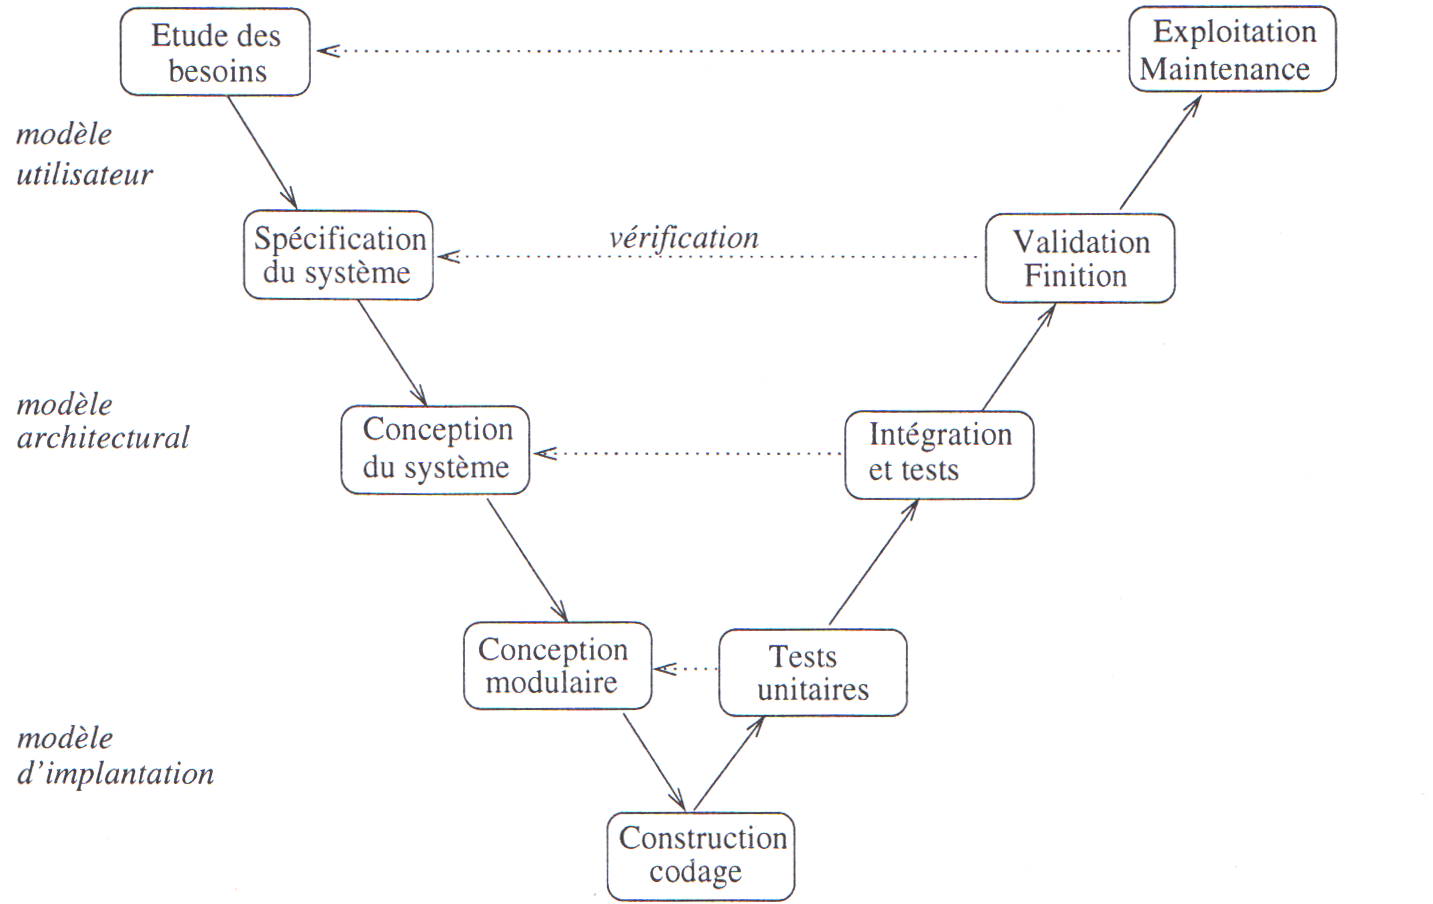
\includegraphics[width=\textwidth]{fig4.png}
\end{framentitle}

\begin{framentitle}{Modèle en spirale (1)}
    \begin{itemize}
        \item 1988 : Boehm
        \item Prise en compte des risques
            \begin{itemize}
                \item Actions pour éviter les risques
            \end{itemize}
        \item 1 cycle :
            \begin{enumerate}
                \item Analyse
                \item Développement du prototype
                \item Essai du prototype
            \end{enumerate}
        \item Dernier cycle : produit fini
    \end{itemize}
\end{framentitle}

% TODO Possibilité d'ajouter la définition de prototype et maquette
\begin{framentitle}{Modèle en spirale (2)}
    \begin{center}
        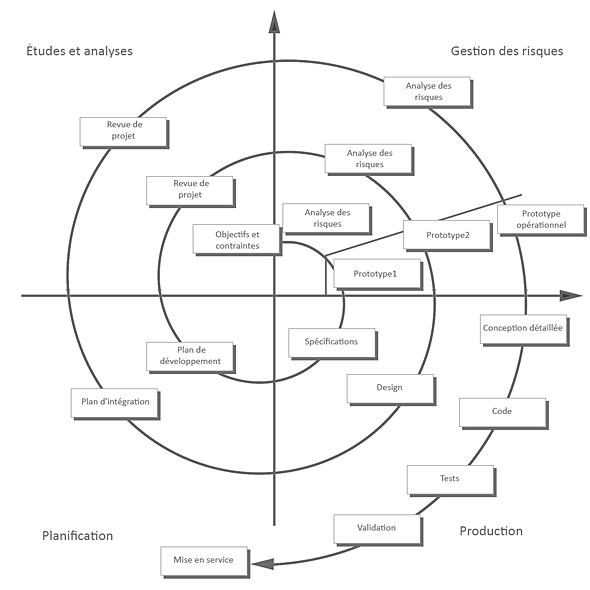
\includegraphics[width=.7\textwidth]{fig7.png}
    \end{center}
\end{framentitle}

\begin{framentitle}{Méthodes agiles}
    \begin{itemize}
        \item Cycle de développement court
        \item Grande réactivité :
            \begin{itemize}
                \item Acceptation du changement
            \end{itemize}
        \item Équipe communicante plus importante que
            les moyens et les outils
        \item Application plus importante que
            la documentation
        \item Collaboration :
            \begin{itemize}
                \item Client impliqué en feed-back continu
            \end{itemize}
    \end{itemize}
\end{framentitle}

\section{Qualité}
% TODO ajouter des exemples de code pour les qualités

\begin{framentitle}{Qualité du logiciel}
    Qualités les plus importantes :
    \begin{itemize}
        \item Validité
            \begin{itemize}
                \item Réaliser exactement les tâches définies par la
                    spécification
            \end{itemize}
        \item Robustesse
            \begin{itemize}
                \item Fonctionne même dans des conditions anormales
            \end{itemize}
        \item Extensibilité
            \begin{itemize}
                \item Facilité d'adaptation du logiciel aux changements de
                    spécification
            \end{itemize}
        \item Réutilisabilité
            \begin{itemize}
                \item Une partie ou le tout peut être réutilisé pour de
                    nouvelles applications
            \end{itemize}
        \item Compatibilité
            \begin{itemize}
                \item Le parties peuvent être combinés
            \end{itemize}
    \end{itemize}
\end{framentitle}

\begin{framentitle}{Critères informatiques (1)}
    Critères permettant d'atteindre ces qualités :
    \begin{itemize}
        \item Modularité
            \begin{itemize}
                \item décomposition en composants simples et indépendants
            \end{itemize}
        \item Complétude
            \begin{itemize}
                \item Degré d'implémentation des spécifications
            \end{itemize}
        \item Cohérence
            \begin{itemize}
                \item Possibilité retour étape de dév. précédente
                \item Ex : remonter une erreur détectée en maintenance au niveau
                    de l'implémentation
            \end{itemize}
    \end{itemize}
\end{framentitle}
\begin{framentitle}{Critères informatiques (2)}
    \begin{itemize}
        \item Généralité
            \begin{itemize}
                \item Plage d'application potentielle des composants
            \end{itemize}
        \item Auto-documentation ou lisibilité
            \begin{itemize}
                \item Possibilité d'extraction de la documentation depuis les
                    composants logiciels
                \item Ex : nom de variables, docstrings, etc.
            \end{itemize}
    \end{itemize}
\end{framentitle}

\begin{framentitle}{Liens qualités $\leftrightarrow$\ critères info.}
    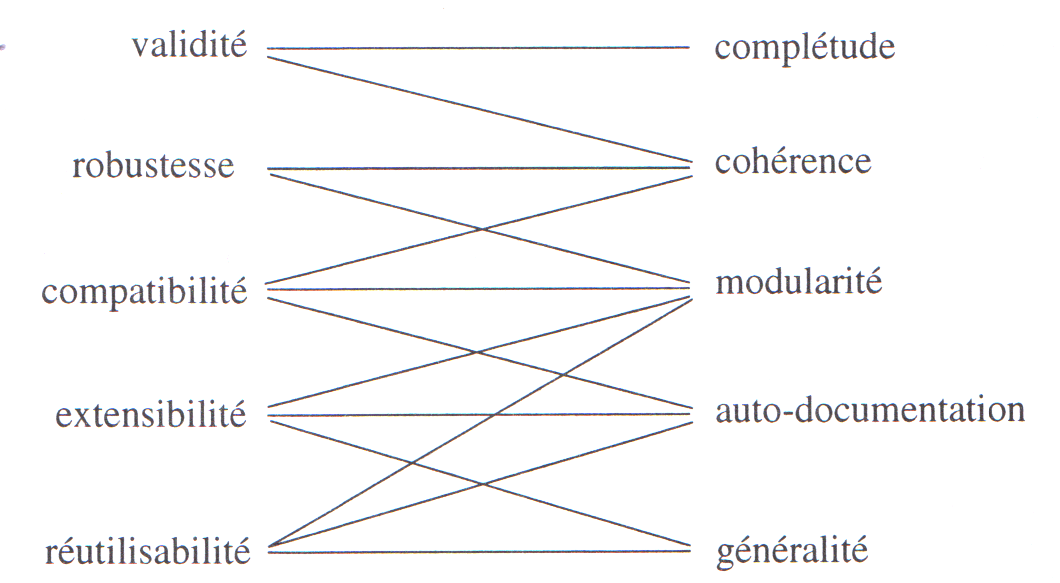
\includegraphics[width=\textwidth]{fig5.png}
\end{framentitle}

\begin{framentitle}{Qualité du proc. de développement (1)}
    Principales qualités :
    \begin{itemize}
        \item Sûreté
            \begin{itemize}
                \item Minimise les retours arrière et validations
                    régulières
            \end{itemize}
        \item Terminaison
            \begin{itemize}
                \item Obtention du produit en temps fini
            \end{itemize}
        \item Rigueur
            \begin{itemize}
                \item Étapes logiques, en accord avec les habitudes des
                    développeurs
            \end{itemize}
        \item Cohérence
            \begin{itemize}
                \item Pas de duplication ou d'oublis
            \end{itemize}
    \end{itemize}
\end{framentitle}

\begin{framentitle}{Qualité du proc. de développement (2)}
    \begin{itemize}
        \item Souplesse
            \begin{itemize}
                \item Adaptation à l'application à développer
            \end{itemize}
        \item Accessibilité
            \begin{itemize}
                \item Comprendre les choix effectués
            \end{itemize}
        \item Rentabilité
            \begin{itemize}
                \item Capitaliser l'expérience
            \end{itemize}
    \end{itemize}
\end{framentitle}

\begin{framentitle}{Critères (1)}
    Critères permettant d'atteindre ces qualités :
    \begin{itemize}
        \item Automatisation
            \begin{itemize}
                \item Moins d'erreur
                \item Plus vite
            \end{itemize}
        \item Réutilisation
            \begin{itemize}
                \item Réduit le coût
                \item Augmente la sureté
            \end{itemize}
        \item Facilité d'écriture
            \begin{itemize}
                \item Modèles simples et naturels pour les développeurs
            \end{itemize}
        \item Guidage
            \begin{itemize}
                \item Opérations à réaliser pour obtenir un bon résultat
            \end{itemize}
        \item Traçabilité
            \begin{itemize}
                \item Vérification de la cohérence entre les modèles
            \end{itemize}
    \end{itemize}
\end{framentitle}

\begin{framentitle}{Critères (2)}
    \begin{itemize}
        \item Contrôle
            \begin{itemize}
                \item Contrôle régulier
            \end{itemize}
        \item Intégration
            \begin{itemize}
                \item Cohérence entre modèles d'une même étape ou deux
                    successives
            \end{itemize}
        \item Documentation
            \begin{itemize}
                \item Raisonnement et choix explicites
            \end{itemize}
        \item Ciblage
            \begin{itemize}
                \item Domaine d'application explicite
            \end{itemize}
        \item Abstraction
            \begin{itemize}
                \item Le raisonnement et la preuve doivent progressivement
                    prendre en compte les concepts de programmation
            \end{itemize}
    \end{itemize}
\end{framentitle}

\begin{framentitle}{Liens qualités $\leftrightarrow$\ critères}
    \begin{center}
        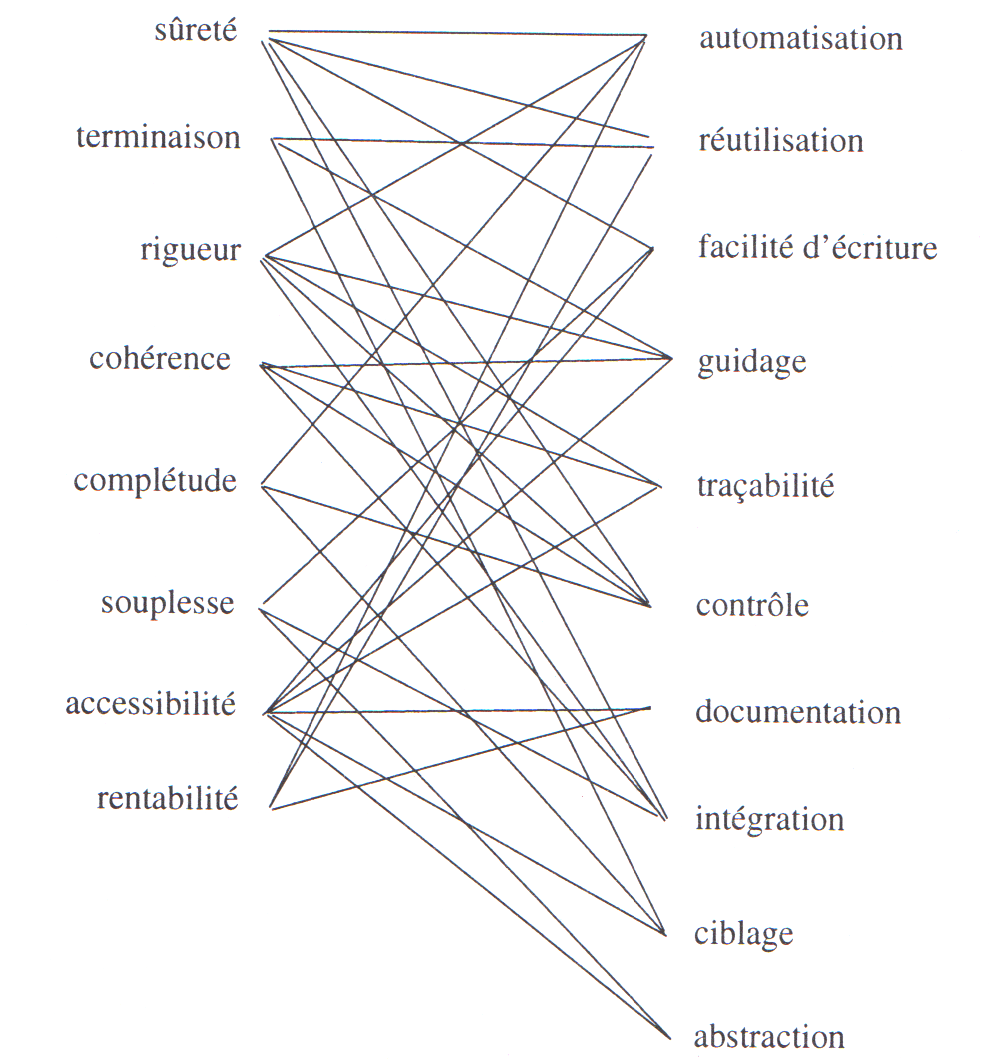
\includegraphics[width=.6\textwidth]{fig6.png}
    \end{center}
\end{framentitle}

\section{Suite du cours}

\begin{framentitle}{Plan de la suite du cours}
    \begin{enumerate}
        \item Merise
            \begin{itemize}
                \item Méthode systémique : vision globale
                \item Modélisation selon l'axe des données
                \item Utilisation pour la modélisation des bases de données
            \end{itemize}
        \item Introduction à UML
            \begin{itemize}
                \item Panel de diagrammes
                    \begin{itemize}
                        \item Approche fonctionnelle, objet (méthode cartésiennes)
                        \item Flot de données
                        \item Possible : modèle de données
                    \end{itemize}
                \item En détail : cas d'utilisation (modélisation fonctionnelle)
            \end{itemize}
        \item Méthodes agiles
    \end{enumerate}
\end{framentitle}

\begin{framentitle}{Trois axes de modélisation}
    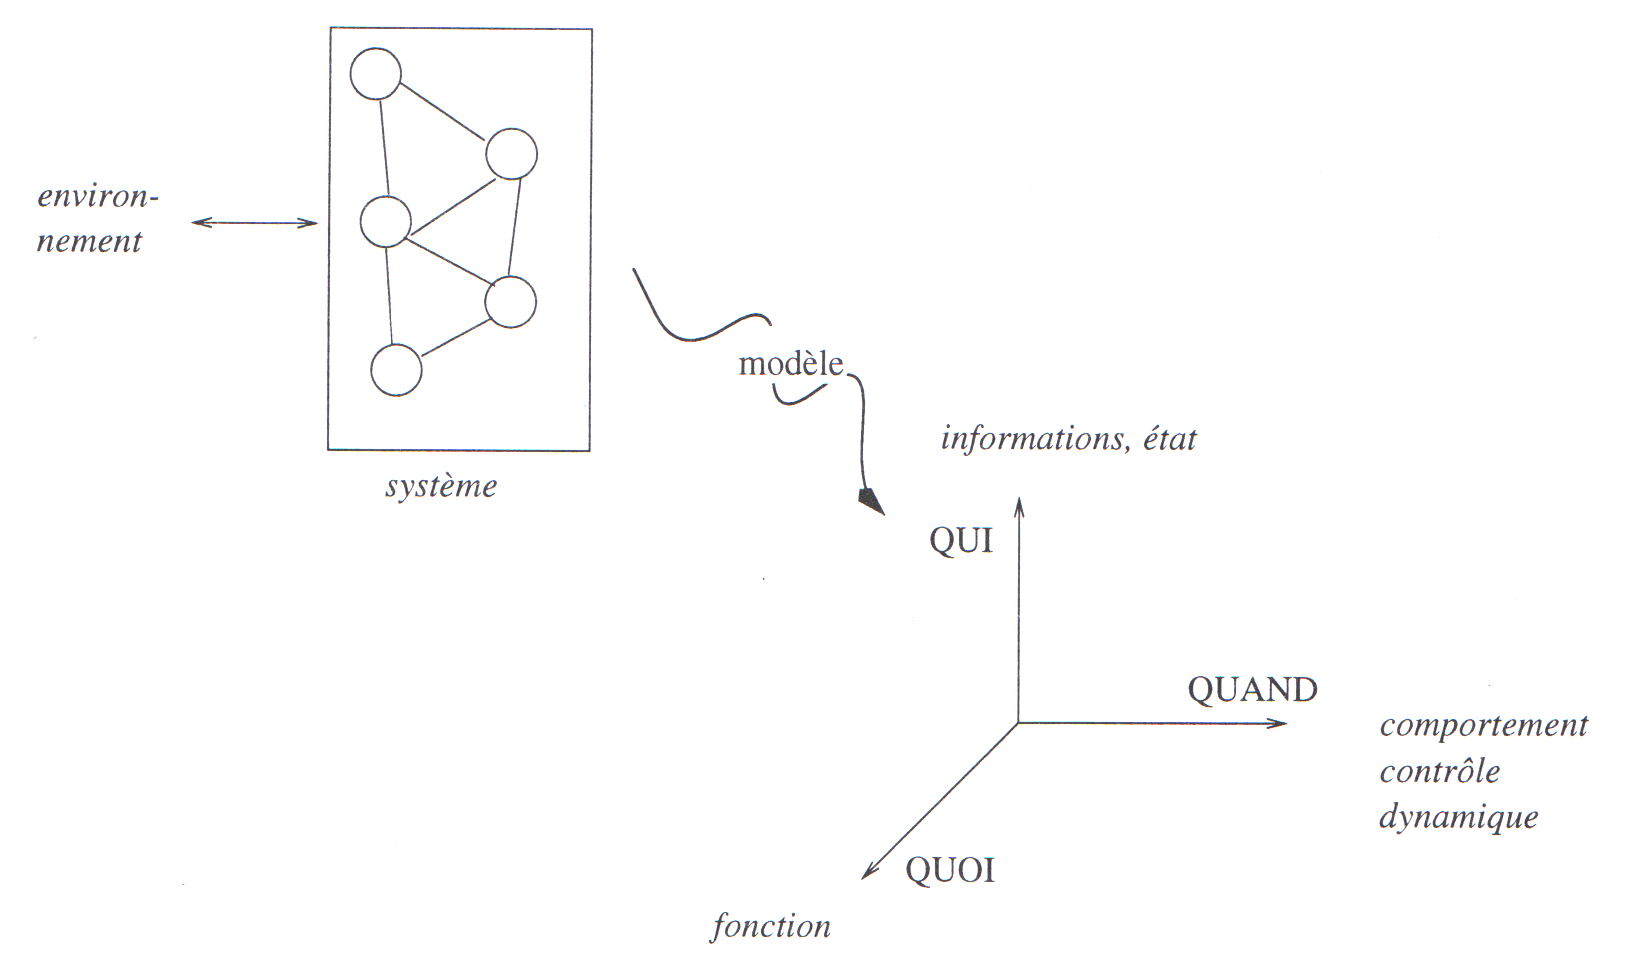
\includegraphics[width=\textwidth]{fig2.png}
    \rae Trois courants de méthodes d'analyse/conception
\end{framentitle}

\begin{framentitle}{Approche fonctionnelle}
    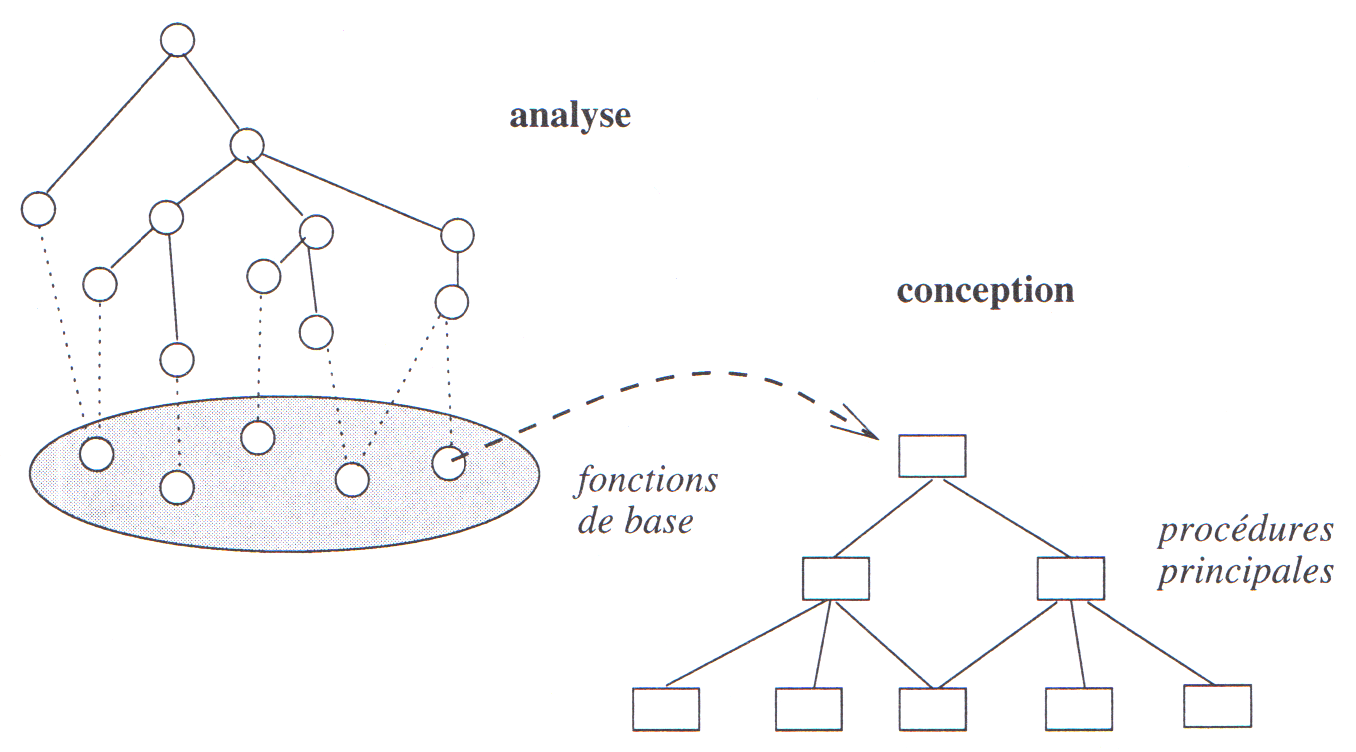
\includegraphics[width=\textwidth]{fig1b.png}
\end{framentitle}

\begin{framentitle}{Approche flots de données}
    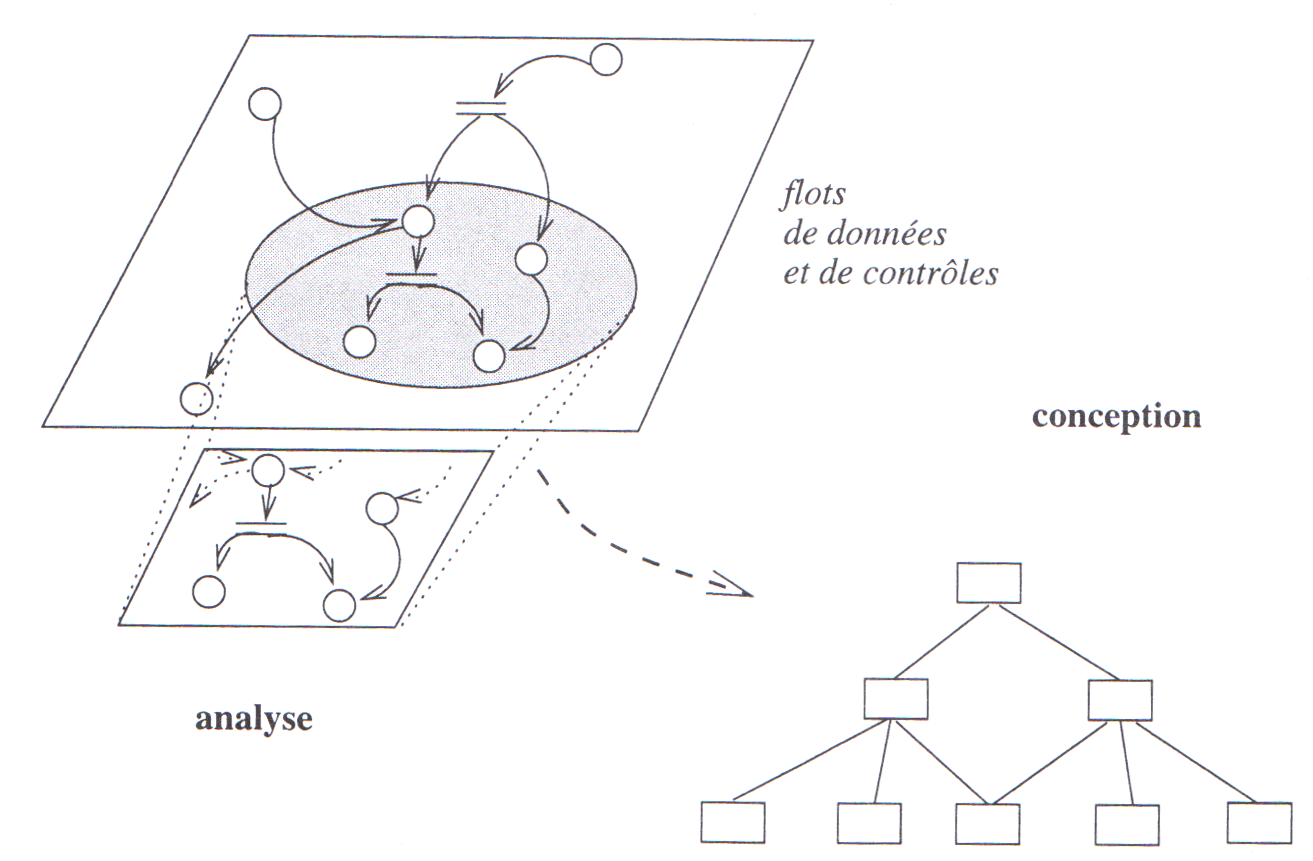
\includegraphics[width=\textwidth]{fig3a.png}
\end{framentitle}

\begin{framentitle}{Approche modèle de données}
    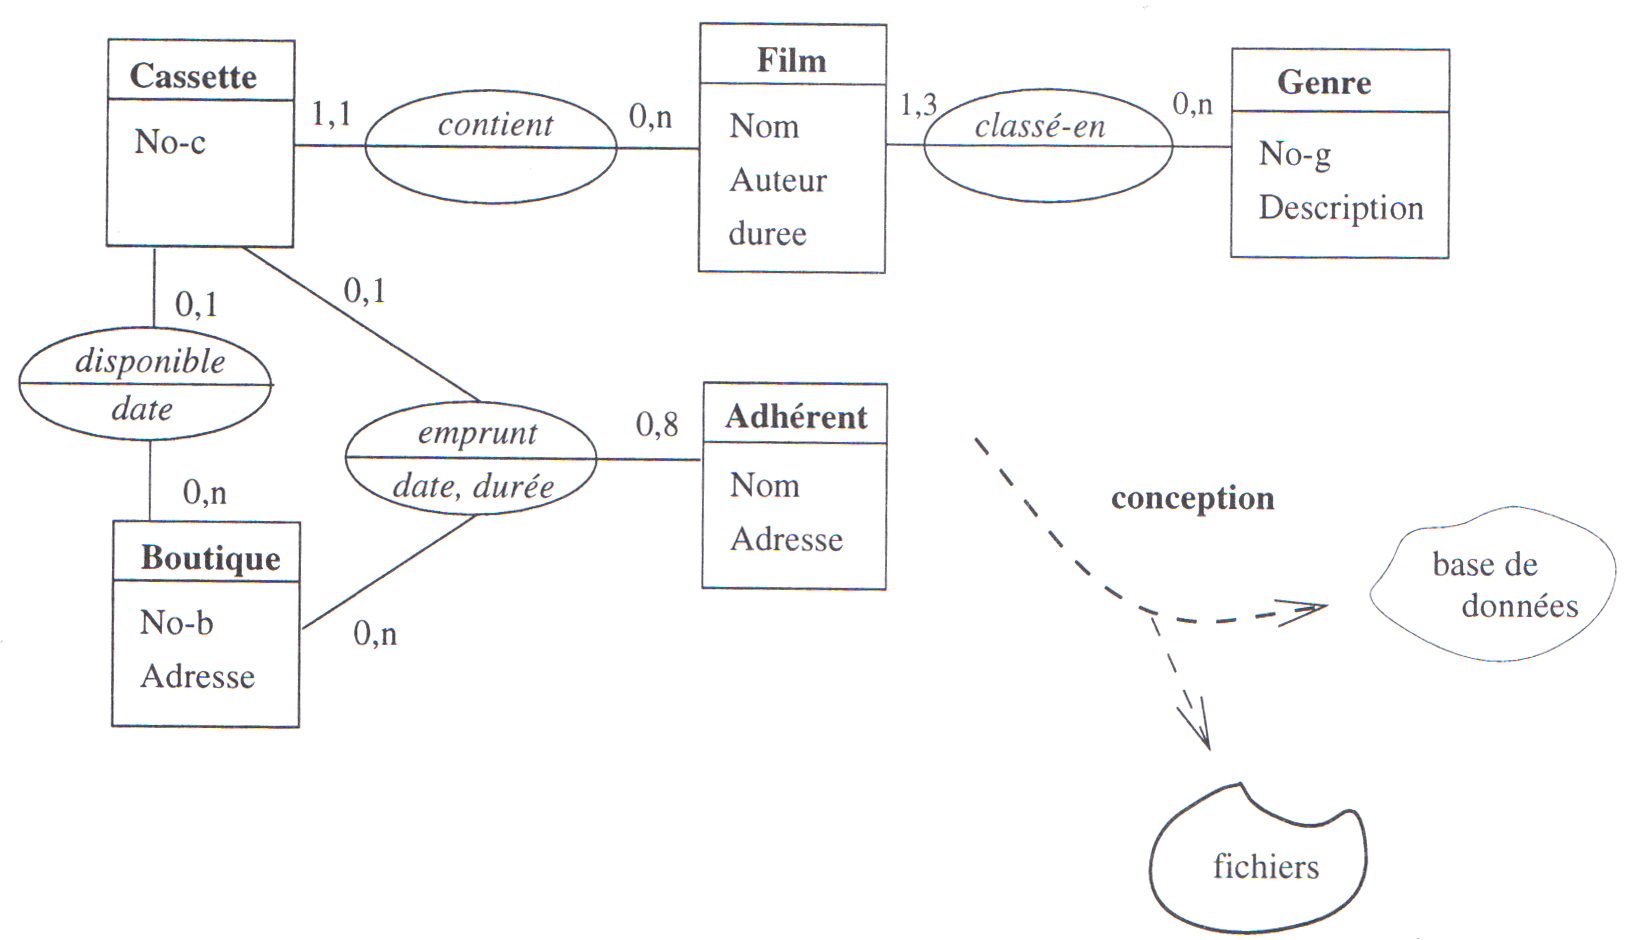
\includegraphics[width=\textwidth]{fig3b.png}
\end{framentitle}

\end{document}
